\usetikzlibrary{positioning,arrows,calc}

\tikzset{
modal/.style={>=stealth’,shorten >=1pt,shorten <=1pt,auto,node distance=1.5cm,
semithick},
world/.style={circle,draw,minimum size=0.5cm,fill=gray!15},
point/.style={circle,draw,inner sep=0.5mm,fill=black},
reflexive above/.style={->,loop,looseness=7,in=120,out=60},
reflexive below/.style={->,loop,looseness=7,in=240,out=300},
reflexive left/.style={->,loop,looseness=7,in=150,out=210},
reflexive right/.style={->,loop,looseness=7,in=30,out=330}
}

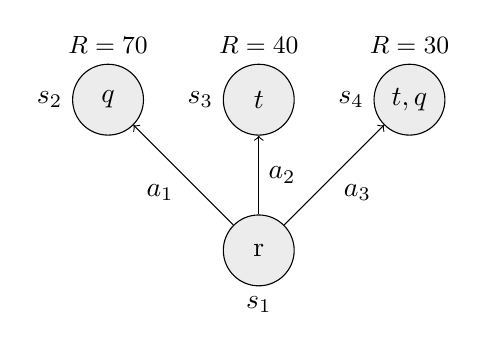
\begin{tikzpicture}[world/.append style={minimum size=0.9cm}]

\node[world] (s1) [label=below:$s_1$] {r};
\node[world] (s3) [label=left:$s_3$,label=above:{\small $R=40$},above=of s1] {$t$};
\node[world] (s2) [label=left:$s_2$,label=above:{\small $R=70$},left=of s3] {$q$};
\node[world] (s4) [label=left:$s_4$,label=above:{\small $R=30$},right=of s3] {$t,q$};


\path[->] (s1) edge node[below left] {$a_1$} (s2);
\path[->] (s1) edge node[right] {$a_2$} (s3);
\path[->] (s1) edge node[below right] {$a_3$} (s4);

\end{tikzpicture}